
\section{FK Analysis} 
\label{sect:fk-analysis}

The FK routines were provided by \textbf{Tormod Kv\ae rna} from NORSAR and 
implemented into SEISAN by \textbf{Andrius Pacesa}. 

\textbf{Some basics}

The FK-analysis\index{FK analysis}, more strictly slowness analysis, is a standard tool in seismic array processing\index{Array processing}. It is used to find the apparent velocity and back azimuth of an incoming wavefront. Apparent velocity can be used to identify the type of wave (P, S, Lg and etc.) and the approximate distance to the source can be determined for teleseimic events. Utilizing azimuth and distance to the source, one can define the approximate location of the signal source. 

A description of frequency-wavenumber analysis - \"f-k analysis\" - may be found in Capon (1969). This method has been further developed to include wide-band analysis and maximum-likelihood estimation techniques - see \citet{kvaerna1986}. 

The principle of slowness analysis is beamforming in the frequency domain for a number of different slowness values and calculating the power for each beam. The beam power will be a maximum in case the slowness of the beam coincides with the slowness of the wavefront crossing an array. So the beam having the maximum power will indicate the slowness of the incoming signal. 

\textbf{Running the program}

The FK program can be started directly with command `fk' or from MULPLT. The program expects that the file `waveform.out' with the seismic traces as input data, is available in the current directory. If the program is invoked directly, this file has to be created before using mulplt, selecting a window and creating the `waveform.out' file. 

In general it is more useful, to start the FK program from MULPLT since the input file needs to be created by mulplt. The result of the fk analysis can be saved to the S-file. 

The steps are: 

\begin{itemize}
\item[-]
start MULPLT 
\item[-]
select channels and a time window 
\item[-]
use option fk to start FK program (this option creates file `waveform.out' and starts FK program), 
accept maximum or pick value with mouse 

The options in FK are: \newline
\verb|                       |R-Redo: Repeat fk analysis with different parameters \newline
\verb|                       |M-Mouse: `m' or mouse click to pick values different from maximum \newline
\verb|                       |S-Save and quit: save picked value to file and quit \newline
\verb|                       |Q-Quit: quit 

\item[-]
use option `save and quit' to save your result, so that it can be used by MULPLT 
\item[-]
back in MULPLT: pick phase on the first trace used, to store back azimuth 
and apparent velocity in the S-file 
\item[-]
in case of teleseismic events, the apparent velocity can be used for location, the fk analysis has to be done on the P phase 
\end{itemize}

Note: The FK program only works by default  with station file `\texttt{STATION0.HYP}'. If coordinates are in e.g. \texttt{STATIONt.HYP}, the user will be asked to specify another station file letter, in this case `t'. 

\textbf{Example}

Input: 

\verbatiminput{include/fk.inp}

Example of output file fk.out: 

\verbatiminput{include/fk.out}

\begin{figure}
\htmlimage{scale=2.0}
\centerline{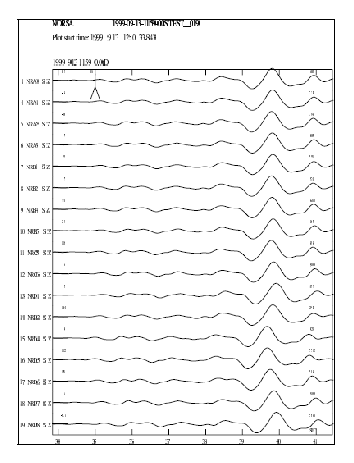
\includegraphics[width=0.9\linewidth]{fig/fig47}}
\caption{The FK program can be started from MULPLT. 
The traces shown were selected and used as input to the FK program. 
The result of the FK analysis is shown in Figure \ref{fig:fk-output}. 
The event shown here is part of the testdata set.}
%\label{fig:}
\end{figure}

\begin{figure}
\htmlimage{scale=2.0}
\centerline{
\includegraphics[width=0.9\linewidth]{fig/fig48}}
\caption{Output from the FK program. Contours and values are the normalized maximum
power.}
\label{fig:fk-output}
\end{figure}

